\documentclass[12pt]{article}

\usepackage{amsmath}
\usepackage{amssymb}
\usepackage{calc}
\usepackage{units}
\usepackage{graphicx}
\usepackage[pdftex]{hyperref}
\usepackage{subfig}
\usepackage[margin=1in]{geometry}
\usepackage{listings}
\usepackage[numbers,sort&compress]{natbib}
\usepackage{bm}
\usepackage{paralist}
\usepackage[draft]{fixme}
\usepackage{textcomp}
\usepackage{menukeys}

\renewmenumacro{\keys}{shadowedroundedkeys}
\renewmenumacro{\menu}[>]{roundedmenus}

\hypersetup{
  breaklinks=true,
  pdftitle={An Introduction to AC Signals and Their Measurement},
  pdfauthor={Kevin R. Lynch},
  pdfsubject={Phyiscs, Electricity and magnetism},
  pdfkeywords={Oscilloscope, Digital Oscilloscope, Signal Generator},
  pdflang={en-US},
}

\title{An Introduction to AC Signals and Their Measurement}
\author{}
%Kevin R. Lynch
%\date{2015-03-25}
\date{}

\begin{document}

\maketitle

\section{Objectives}
\label{sec:objectives}

\begin{enumerate}
\item To understand the basics of alternating currents in resistive
  circuits,
\item To learn the operation of a modern digital oscilloscope,
\item To learn to generate AC voltages with a modern digital function
  generator, and
\item To measure AC voltages, and the amplitude and frequency
  of a waveform with an oscilloscope and multimeter.
\end{enumerate}

\section{Introduction}
\label{sec:introduction}

To date, we have looked at the behavior of constant voltage sources in
purely resistive circuits: Ohm's Law, equivalent resistance, and
Kirchoff's rules.  Of course constant voltages drive constant
currents, and these types of systems are known as \textit{Direct
  Current} or DC systems.  DC systems aren't very interesting: you
can't do much more than deliver power with DC.  You certainly can't do
the types of things we really \textit{want} electrical circuits to do,
like sample the world, manipulate information, play video games, etc.

Circuits with changing voltages are called generically
\textit{Alternating Current}, or AC systems.  DC signals are
characterized by a single number: the voltage above the ground
reference (aka ``the voltage'').  AC signals, however, don't have this
property; they can be literally \textit{anything}.  Throughout the
rest of the semester, we will spend most of our time studying a
particular type of AC signal, the sinusoid or sine wave signal, which
isn't quite so wild and unconstrained.  We'll do this because of
Fourier's Theorem, which tells us that any periodic signal can be
decomposed into a sum of sinusoids.  Understanding the behavior of
pure sinusoids allows us to understand the behavior of significantly
more complicated signals with relative ease.

To probe and understand AC signals, we require new tools and
techniques beyond DC power supplies and multimeters.  There are many
tools and devices to generate AC signals, but all of them can be
considered as new types of power supplies.  In this course, we will be
using a fairly simple type called a \textit{function} or
\textit{signal generator}.

Similarly, there are many, many different types tools to measure AC
signals.  We will use two of the most generically useful devices: our
trusty multimeters, and a specialized form of voltmeter called an
\textit{oscilloscope}.  Although we will use them extensively, the
multimeter is rather a limited tool for AC measurements: it measures
moments of the signal (also known as descriptive statistics; think
``averages''), not the global structure or details of the signal.  If
you don't already know what the signal looks like, the measurements
out of the multimeter aren't going to tell you anything useful.  That
said, if you \textit{do} know what the signal looks like, there are
few general purpose tools that will give you more accurate
measurements than a good benchtop digital multimeter.  In particular,
we will be using the multimeter to measure the \textit{frequency} of
periodic signals (sinusoids, square waves, etc), as well at the
\textit{RMS voltage} or \textit{RMS current} of the signal.  The
latter is the ``root mean square'' of the signal: take the signal,
\textit{square} it so that it is always positive, take the average or
\textit{mean} of that new signal, then take the square \textit{root}
of the result.  For periodic signals whose averages are zero, the RMS
gives a meaningful measurement of the size of the waveform.  For a
sinusoid in particular, the RMS voltage is $1/\sqrt{2}$ smaller than
the amplitude, which itself is half the peak-to-peak voltage (the
difference between the maximum and minimum voltage):
\begin{align*}
  V_\text{RMS} &= \frac{1}{\sqrt{2}} V_\text{amp} & V_\text{amp} &= V_\text{pp}\ . 
\end{align*}

From an operating perspective, you should think of oscilloscopes as
nothing more than really fancy voltmeters: if you already know how to
measure signals with a multimeter, you connect an oscilloscope to the
circuit in the same way.  On the other hand, oscilloscopes can give
you a detailed, visual picture of the entire profile of the signal, not
just moment information.  Where the multimeter can measure with
fantastic accuracy \textit{if} you know the form of the signal, the
oscilloscope is the tool that \textit{tells} you what that form is.
Inside the shell, a modern digital oscilloscope is usually nothing
more than a commodity personal computer with specialized electronic
measurement peripherals, a specialized interface, and specialized
software to simultaneously measure and display dozens of parameters of
the input signals.  We'll touch on a number of those measurements in
this lab.

There is another key difference between a multimeter and an
oscilloscope that bears mentioning here.  Multimeters usually can only
measure one signal at a time, while oscilloscopes usually have more
(ours can measure four).  On the other hand, multimeters have
\textit{floating} inputs; that is, they directly measure the voltage
difference between the two inputs, which can be connected to
\textit{any} two points in the circuit.  Oscilloscopes have
non-floating inputs: the \textit{reference} or \textit{ground} sides
of each channel are tied together, and are tied to the \textit{chassis
  ground} (also known as \textit{earth ground} or \textit{safety
  ground}) of the device, which is always connected to the ground lead
on the power cord.  The grounds of all channels have to be connected
to the same point in the circuit, and you are usually forced to make
that point the same as the ground terminal of the power supply.  To
measure the voltage between two arbitrary points using an oscilloscope
requires simultaneous measurements on two channels, and a subtraction
operation.  We'll show you how to do this later on in this lab.

We will only just barely scratch the outer surface of what these
devices can do in this lab; I urge you to read through some of the
overviews and tutorials linked in Section~\ref{sec:references} before
coming to lab, and to keep them handy throughout the rest of the
semester. 

\section{Procedures}
\label{sec:procedures}

In this lab, you will use some equipment you are already familiar with
(the Agilent U3401A multimeter) in unfamiliar ways, and some new
equipment (the Teledyne Lecroy WaveAce 2014 Digital Oscilloscope and
the Tektronix AFG2021 Function Generator).  You will also need a
resistance board, some BNC-to-banana plug adapters, and the standard
banana plug cables.

Remember that the goal of this lab is to learn to use the equipment
with proficiency, not to test any hypothesis.  While this equipment is
relatively simple for modern equipment, these devices are packed with
dozens of features, most of which you will never need to use in this
course.  You would do yourself a favor, and really \textit{read} the
documents linked in Section~\ref{sec:references}.  Also, the manuals
for the oscilloscopes are available from the CLTs; please request to
borrow them if you think it will help.  The manual is also linked in
Section~\ref{sec:references}.

\begin{figure}
  \centering
  \includegraphics[width=\textwidth/2]{figures/tektronix_afg2021}
  \caption{The front panel of the AFG2021 Function Generator.}
  \label{fig:funcgen}
\end{figure}
\begin{figure}
  \centering
  \includegraphics[width=\textwidth/2]{figures/teledyne_lecroy_waveace2014}
  \caption{The front panel of the WaveAce 2014 Digital Oscilloscope.}
  \label{fig:oscope}
\end{figure}
\begin{figure}
  \centering
  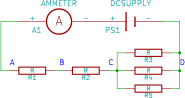
\includegraphics[width=\textwidth/3]{figures/circuit}
  \caption{The circuit used for this training exercise.  V1 is the
    function generator (a \textit{voltage} source), while R1 and R2
    are resistors. Do not build this circuit until instructed to do so
    by the instructions!}
  \label{fig:circuit}
\end{figure}
\begin{figure}
  \centering
  \includegraphics[width=\textwidth/3]{figures/measuring}
  \caption{How to measure the voltage across a device with an
    oscilloscope; see the text in Section~\ref{sec:oscope}.}
  \label{fig:measuring}
\end{figure}

\subsection{Measure the Resistors}
\label{sec:resistors}

\begin{enumerate}
\item Let's start by choosing two resistors on your board, and
  measuring and recording their resistances with the multimeter.
\end{enumerate}

\subsection{Prepare the Function Generator}
\label{sec:funcgen}

\begin{enumerate}
\item Next, we'll set up the AFG2021 (see Figure~\ref{fig:funcgen}):
  \begin{compactenum}
  \item Turn on the power by pressing the \keys{On} button.  Because
    the AFG2021 is microprocessor controlled, it needs to boot up and
    run a series of self tests and calibrations. Be patient; it only
    takes a few seconds.
  \item Press the \keys{Sine} button to select a sinusoidal voltage
    profile, then press \keys{Continuous} to ensure a continuous,
    non-triggered output waveform.
  \item Next we have to set the frequency of the generated function;
    you will need to use the softkeys to the right of the screen, and
    the keypad.  Select the \menu{Frequency,Period,Phase
      Menu>Frequency}, enter a frequency on the keypad, and then press
    the appropriate Unit softkey.  For example, to set \unit[9]{kHz},
    press \keys{9} then the \menu{kHz} softkey.  For this lab, select
    a value between \unit[5]{kHz} and \unit[10]{kHz}.  To return to
    the main softkeys menu, you need to press the \keys{\arrowkeyup}
    key to back out one level.
  \item Since we don't want a signal that is either too big or too
    small in amplitude, we have to set the amplitude of the signal.
    Again, we go through the softkeys: select \menu{Amplitude,Level
      Menu>Amplitude}, enter a value on the keypad, and select the
    \menu{Vpp} softkey.  For this lab, you should enter
    $\unit[2]{V_{pp}}$; no more, no less please.  Again, you will need
    to press the \keys{\arrowkeyup} key to back out to the main menu.
  \item Wire the circuit shown in Figure~\ref{fig:circuit}.  Make sure
    you connect the circuit to the leftmost Channel connector, not the
    Trigger Output connector in the middle.  If you do, you are going
    to be very confused as to what is going on \ldots You will need to
    connect a ``BNC-to-banana'' adapter to the Channel output.
  \item Now that the circuit and function generator are set up, you
    need to turn the Channel Output on, or you won't measure any
    signal.  Press the \keys{Channel On/Off} to enable the output;
    when the button is lit, the output should be enabled.
  \end{compactenum}
\end{enumerate}

\subsection{Measurements with the Multimeter}
\label{sec:multimeter}

\begin{enumerate}
\item Power on the multimeter, and set it to measure AC Voltage by
  pressing the \keys{ACV} button.
\item With an oscillating voltage, of course, there is no sensible
  ``sign'' of the voltage - it switches polarity every half cycle.  So
  it doesn't matter which input goes on which side of the device or
  voltage source.
\item Measure and record the AC Voltage drop across the function
  generator, and both resistors.  Is Kirchoff's Loop rule satisfied
  here? 
\item Compare the multimeter measured voltage (RMS!) across the
  function generator to the voltage you set (peak-to-peak!).  How do
  they compare?
\item Next, set the multimeter to measure the frequency of the signal
  by pressing the \keys{Freq} button.  Notice that the device screen
  displays two outputs: the frequency on the main portion of the
  display, and the voltage in the upper right.  Measure as if you were
  using a multimeter.  How many places do you need to measure the
  frequency?  How does the measured frequency compare to the frequency
  you set on the function generator in the previous section?
\end{enumerate}

\subsection{Measurements with the Oscilloscope}
\label{sec:oscope}

As we mentioned before, digital oscilloscopes are both fancy
voltmeters, and powerful data processing computers.  We'll exercise
some of the feature of the ``scope'' in this section.

\begin{enumerate}
\item Let's start with something simple: connect the ``GND'' (black)
  side of the output adapter on the function generator to the ``GND''
  side of the oscilloscope's Channel 1 input; see
  Figure~\ref{fig:oscope}.
\item Press the ``magical'' \keys{AUTO} button.  You will hear a
  number of relays clicking and popping inside the device.  When that
  all stops, you should see a number of cycles of a sinusoidal
  waveform on the display.
\item Play with the knobs!  Start with the \keys{Horizontal} knobs on
  the upper right.  The larger knob affects the ``time per division''
  or the horizontal timescale, while the smaller knob moves the
  trigger point (and hence the waveforms) left and right on the
  screen.  There are independent \keys{Vertical} knobs for each
  channel.  Again, the larger knob affects the ``volts per division''
  or the vertical timescale, while the smaller knob moves the ``ground
  reference'' or ``baseline'' up and down on the screen.  The smaller
  knobs are continuously variable, while you should feel the detents
  for the larger knobs.  Each ``click'' of the large knobs changes a
  horizontal or vertical scale factor, and there is a corresponding
  scale displayed on the display; find those scale factors, and
  understand how they relate to changes in the knobs.
\item Now we want to measure something, and there are a number of ways
  to do that.  First, let's use the ``measurement'' features of the
  scope.  In the \keys{Menu Control} block in the upper half of the
  controls, press the \keys{Measure} button.  A vertical menu will
  appear on the right side of the display next to the softkeys.  You
  can set up a number of automatic measurements that will be done
  continuously on a given channel.  Play with the options in the menu,
  until you are simultaneously measuring peak-to-peak voltage,
  frequency, and period for Channel 1.  How do these compare to the
  output settings on the function generator?  To the measurements you
  made with the multimeter?
\item Let's use the second measurement method built into the scope:
  cursors.  The cursor feature allows you to mark a pair of features
  on the screen, and measure the horizontal (time) or vertical
  (voltage) difference between them.  This is most useful for
  non-sinusoidal features, but we'll continue to use the sine wave for
  pedagogical reasons.  
\item Finally, the third measurement method is built into the
  operator: the Mark I Eyeball.  You can make quick measurements in
  the vertical and horizontal directions by counting the number of
  grid marks between the features of interest, and multiplying by the
  scale factor displayed on screen.  Try now to measure the period and
  peak-to-peak voltage ``by eye''.
%\item \fxfatal{triggers}
%\item \fxfatal{acquire menu for averaging}
\item As we mentioned before, unlike the ``floating'' inputs of the
  multimeter (which can directly measure the voltage difference
  between any two points in the circuit), the inputs on the
  oscilloscope are tied to each other and to the ``earth'' or power
  system ground, so they can't directly measure the voltage difference
  between any two arbitrary points.  What they measure is the
  difference between the ground reference and any other point in the
  circuit.  It \textit{is} possible to measure the voltage between any
  two arbitrary points, by using two channels and \textit{subtracting}
  the measured signals at those two points.\footnote{There is one
    complication that we won't have to worry about in these labs:
    signal time delays in the cables connecting the circuit to the
    oscilloscope.  Out signals are slow enough that this isn't going
    to be a problem, but can be with much higher frequency signals.}
  We'll measure the voltage across the two resistors using two
  reference points.  Connect Channels 1 and 2 as shown in
  Figure~\ref{fig:measuring}, and turn on Channel 2 by pressing the
  \keys{CH 2} button above the second input; it should light up, and a
  second trace should appear on the display.  To measure the voltage
  profile across Resistor 1, we need to subtract the two measured
  voltages, since neither end of Resistor 1 is at ground potential.
  Press the \keys{Math} button, just below and between the large knobs
  for Channels 2 and 3.  Using the softkeys to the right of the
  display, choose the \keys{Operation} to be \keys{$A-B$}, set
  \keys{Source A} to Channel 1, and \keys{Source B} to Channel 2.
\item Using the \keys{Measure} or \keys{Cursors} menus, you can
  measure the \keys{Math} trace for peak-to-peak voltage, or
  frequency, etc.  Do so now.
\end{enumerate}

Our oscilloscopes are capable of much more than we have covered here;
we'll introduce some additional features in the future as we need
them. 

\section{References}
\label{sec:references}

In the electronic PDF version of this document, the following list of
references links to the online version of the resource:
\begin{compactitem}
\item
  \href{https://learn.sparkfun.com/tutorials/how-to-use-an-oscilloscope}{The
    Sparkfun tutorial \textit{How to Use an Oscilloscope}}
\item
  \href{http://ecee.colorado.edu/~mcclurel/txyzscopes.pdf}{Tektronix'
    \textit{The XYZ's of Oscilloscopes}}
\item \href{http://teledynelecroy.com/doc/docview.aspx?id=7670}{The
    Teledyne LeCroy \textit{WaveAce 1000/2000 Operator's Manual}}
\item \href{http://teledynelecroy.com/resources/details.aspx?doctypeid=23&mseries=402}{Teledyne LeCroy Tutorials for the WaveAce Oscilloscopes}
\end{compactitem}


\begin{comment}
  \newpage

  \section*{Pre-Lab Exercises}

  Answer these questions as instructed on Blackboard; make sure to
  submit them before your lab session!

  \begin{enumerate}
  \item Download and read some of the documents listed in
    Section~\ref{sec:references}.
  \item The resistance between the input terminals of an oscilloscope
    are very large.  Does that make it more like a voltmeter or more
    like an ammeter?  Why?  Do you make measurements in parallel or in
    series with the circuit elements?
  \item The Oscilloscope has two display axes.  What quantities are
    typically displayed on the two axes in sweep mode?
  \item Describe how to measure the amplitude of a sine wave signal in
    sweep mode.  How does that differ from the peak-to-peak and RMS
    voltages?
  \item Describe how to measure the frequency of a sine wave signal in
    sweep mode.
  \item What is meant by triggering?
  \end{enumerate}
\end{comment}

  \newpage

  \section*{Post-Lab Exercises}

  Unusually, there are no post lab exercises for this lab.  Enjoy your
  spring break!

\end{document}

%%% Local Variables: 
%%% mode: latex
%%% TeX-master: t
%%% End: 
